\chapter{Surrogate Models}\label{Chap:SurMod}
This chapter deals with the theory behind Dakota's surrogate models, which 
are also known as response surfaces and meta-models.

\section{Kriging and Gaussian Process Models}\label{Sec:KrigGP}

In this discussion of Kriging and Gaussian Process (GP) models, vectors are 
indicated by a single underline and matrices are indicated by a double 
underline.  Capital 
letters indicate data, or functions of data, that is used to construct 
an emulator.  Lower case letters indicate arbitrary points, i.e. points
 where the simulator may or may not have been evaluated, and functions 
of arbitrary points. Estimates, approximations, and models are indicated 
by hats.  For instance, $\hat{f}\left(\underline{x}\right)$ is a 
model/emulator of the function $f\left(\underline{x}\right)$ and 
$\hat{y}$ is the emulator's prediction or estimate of the true response 
$y=f(\underline{x})$ evaluated at the point $\underline{x}$.  A tilde 
indicates a reordering of points/equations, with the possible omission of 
some but not all points. $N$ is the number of points in the sample design 
and $M$ is the number of input dimensions.

\subsection{Kriging \& Gaussian Processes: Function Values Only}
\label{SubSec:KrigGP}
The set of interpolation techniques known as Kriging, also referred to 
as Gaussian Processes, were originally developed in the geostatistics 
and spatial statistics communities to produce maps of underground 
geologic deposits based on a set of widely and irregularly spaced 
borehole sites\cite{Cre91}. Building a Kriging
model typically involves the
\begin{enumerate}
\item Choice of a trend function,
\item Choice of a correlation function, and
\item Estimation of correlation parameters.
\end{enumerate}

A Kriging emulator, 
$\hat{f}\left(\underline{x}\right)$, consists of a trend function 
(frequently a least squares fit to the data,
$\underline{g}\left(\underline{x}\right)^T\underline{\beta}$) plus a 
Gaussian process error model, $\epsilon\left(\underline{x}\right)$, 
that is used to correct the trend function.
\begin{displaymath}
\hat{f}\left(\underline{x}\right)=\underline{g}\left(\underline{x}\right)^T\underline{\beta}+\epsilon\left(\underline{x}\right)
\end{displaymath}
This represents an estimated distribution for the unknown true surface,
$f\left(\underline{x}\right)$.  The error model, 
$\epsilon\left(\underline{x}\right)$, makes an adjustment to the
trend function so that the emulator will interpolate, and have zero
uncertainty at, the data points it was built from.   The covariance 
between the error at two arbitrary points, $\underline{x}$
and $\underline{x'}$, is modeled as 
\begin{displaymath}
{\rm Cov}\left(y\left(\underline{x}\right),y\left(\underline{x'}\right)\right)={\rm Cov}\left(\epsilon\left(\underline{x}\right),\epsilon\left(\underline{x'}\right)\right)=\sigma^2\ r\left(\underline{x},\underline{x'}\right).
\end{displaymath}
Here $\sigma^2$ is known as the unadjusted variance and 
$r\left(\underline{x},\underline{x'}\right)$ is a correlation function. 
Measurement error can be modeled explicitly by modifying this to
\begin{displaymath}
{\rm Cov}\left(\epsilon\left(\underline{x}\right),\epsilon\left(\underline{x'}\right)\right)=\sigma^2\ r\left(\underline{x},\underline{x'}\right)+\Delta^2\delta\left(\underline{x}-\underline{x}'\right)
\end{displaymath}
where 
\begin{displaymath}
\delta\left(\underline{x}-\underline{x}'\right)=\left\{\begin{tabular}{ll} 1 & if $\underline{x}-\underline{x}'=\underline{0}$ \\ 0 & otherwise \end{tabular} \right.
\end{displaymath}
and $\Delta^2$ is the variance of the measurement error.  In this work, 
the term ``nugget'' refers to the ratio 
$\eta=\frac{\Delta^2}{\sigma^2}$.\newline

By convention, the terms simple Kriging, ordinary Kriging, and universal 
Kriging are used to indicate the three most common choices for the trend
function.  In simple Kriging, the trend is treated as a known constant, 
usually zero, $g\left(\underline{x}\right)\beta\equiv 0$.  Universal 
Kriging \cite{Mat71} uses a general polynomial trend model 
$\underline{g}\left(\underline{x}\right)^T\underline{\beta}$ whose 
coefficients are determined by least squares regression. Ordinary Kriging
is essentially universal Kriging with a trend order of zero, i.e. the 
trend function is treated as an unknown constant and 
$g\left(\underline{x}\right)=1$. $N_{\beta}$ is the number of basis
functions in $\underline{g}\left(\underline{x}\right)$ and therefore
number of elements in the vector $\underline{\beta}$.\newline

For a finite number of sample points, $N$, there will be uncertainty
about the most appropriate value of the vector, $\underline{\beta}$, 
which can therefore be described as having a distribution of possible
values.  If one assumes zero prior knowledge about this distribution, 
which is referred to as the ``vague prior'' assumption, then the maximum
likelihood value of $\underline{\beta}$ can be computed via least 
squares generalized by the inverse of the error model's correlation 
matrix, $\underline{\underline{R}}$ 
\begin{displaymath}
\underline{\hat{\beta}}=\left(\underline{\underline{G}}^T\underline{\underline{R}}^{-1}\underline{\underline{G}}\right)^{-1}\left(\underline{\underline{G}}^T\underline{\underline{R}}^{-1}\underline{Y}\right).
\end{displaymath}
Here $\underline{\underline{G}}$ is a $N$ by $N_\beta$ matrix that 
contains the evaluation of the least 
squares basis functions at all points in $\underline{\underline{X}}$, 
such that $G_{i,l}=g_l\left(\underline{X_i}\right)$.  The real, symmetric, 
positive-definite correlation matrix, $\underline{\underline{R}}$, of the 
error model contains evaluations of the correlation function, $r$, at all 
pairwise combination of points (rows) in the sample design, 
$\underline{\underline{X}}$.
\begin{displaymath}
R_{i,j}=R_{j,i}=r\left(\underline{X_i},\underline{X_j}\right)=r\left(\underline{X_j},\underline{X_i}\right)
\end{displaymath}

There are many options for $r$, among them are the following 
families of correlation functions:
\begin{itemize}
\item {\bf Powered-Exponential}
      \begin{equation}
        r\left(\underline{X_i},\underline{X_j}\right)=\exp\left(-\sum_{k=1}^M \theta_k\left|X_{i,k}-X_{j,k}\right|^\gamma\right)
        \label{Eqn:PowExpCorrFunc}
      \end{equation}
      where $0<\gamma\le2$ and $0<\theta_k$.
\item {\bf Matern}
      \begin{displaymath}
        r\left(\underline{X_i},\underline{X_j}\right)=\prod_{k=1}^M \frac{2^{1-\nu}}{\Gamma(\nu)}\left(\theta_k\left|X_{i,k}-X_{j,k}\right|\right)^\nu\mathcal{K}_\nu\left(\theta_k\left|X_{i,k}-X_{j,k}\right|\right)
      \end{displaymath}
      where $0<\nu$, $0<\theta_k$, and $\mathcal{K}_\nu(\cdot)$ is the 
      modified Bessel function of order $\nu$; $\nu=s+\frac{1}{2}$ is  
      the smallest value of $\nu$ which results in a Kriging model that 
      is $s$ times differentiable. 
\item {\bf Cauchy}
      \begin{displaymath}
        r\left(\underline{X_i},\underline{X_j}\right)=\prod_{k=1}^M \left(1+\theta_k\left|X_{i,k}-X_{j,k}\right|^\gamma\right)^{-\nu}
      \end{displaymath}
      where $0<\gamma\le2$, $0<\nu$, and $0<\theta_k$.
\end{itemize}
Gneiting et al. \cite{Gne07} provide a more 
thorough discussion of the properties of and relationships between these
three families.  Some additional correlation functions include the 
Dagum family \cite{Ber08} and cubic splines.\newline

The squared exponential or Gaussian correlation function (Equation 
\ref{Eqn:PowExpCorrFunc} with $\gamma=2$) was selected to be the 
first correlation function implemented in Dakota on the basis that 
its infinite smoothness or differentiability should aid in leveraging 
the anticipated and hopefully sparse data.
For the Gaussian correlation function, the correlation parameters, 
$\underline{\theta}$, are related to the correlation lengths, 
$\underline{L}$, by
\begin{equation}
\theta_k=\frac{1}{2\ L_k^2}.
\end{equation}
Here, the correlation lengths, $\underline{L}$, are analogous to 
standard deviations in the Gaussian or normal distribution and often 
have physical meaning. The adjusted (by data) mean of the emulator is 
a best linear unbiased estimator of the unknown true function,
\begin{equation}
\hat{y}={\rm E}\left(\hat{f}\left(\underline{x}\right)|\underline{f}\left(\underline{\underline{X}}\right)\right)=\underline{g}\left(\underline{x}\right)^T\underline{\hat{\beta}}+\underline{r}\left(\underline{x}\right)^T\ \underline{\underline{R}}^{-1}\underline{\epsilon}.
\label{Eq:KrigMean}
\end{equation}
Here, $\underline{\epsilon}=\left(\underline{Y}-\underline{\underline{G}}\ \underline{\hat{\beta}}\right)$ 
is the known vector of differences between the true outputs and trend 
function at all points in $\underline{\underline{X}}$ and the vector 
$\underline{r}\left(\underline{x}\right)$ is defined such that
$r_i\left(\underline{x}\right)=r\left(\underline{x},\underline{X_i}\right)$.  
This correction can be interpreted as the projection of prior belief 
(the least squares fit) into the span of the data. The adjusted mean 
of the emulator will interpolate the data that the Kriging model was 
built from as long as its correlation matrix, $\underline{\underline{R}}$, 
is numerically non-singular.\newline

Ill-conditioning of $\underline{\underline{R}}$ and other matrices
is a recognized as a significant challenge for Kriging. Davis and 
Morris \cite{Dav97} gave a thorough review of six factors 
affecting the condition number of matrices associated with Kriging
(from the perspective of semivariograms rather than correlation 
functions).  They concluded that 
``Perhaps the best advice we can give is to be mindful of the 
condition number when building and solving kriging systems.''\newline


In the context of estimating the optimal $\underline{\theta}$,
Martin \cite{Mar09} stated that Kriging's
``three most prevalent issues are (1) ill-conditioned correlation 
matrices,(2) multiple local optimum, and (3) long ridges of near 
optimal values.'' Because of the second issue, global optimization 
methods are more robust than local methods.  Martin used constrained 
optimization to address ill-conditioning of $\underline{\underline{R}}$.
\newline

Rennen \cite{Ren09} advocated that ill-conditioning
be handled by building Kriging models from a uniform subset of 
available sample points.  That option has been available in
Dakota's ``Gaussian process'' model (a separate implementation 
from Dakota's ``Kriging'' model) since version 4.1~\cite{UserMan4_1}. 
Note that Kriging/Gaussian-Process models 
will not exactly interpolate the discarded points.  The implicit 
justification for this type of approach is that the row or columns of 
an ill-conditioned matrix contain a significant amount of duplicate 
information, and that when discarded, duplicate information should be 
easy to predict.\newline  

As of version 5.2, Dakota's \texttt{kriging} model has a similar 
``discard near duplicate points'' capability.  However, it explicitly
addresses the issue of unique information content.  Points are {\bf not} 
discarded prior to the construction of the Kriging model.  Instead,
for each vector $\underline{\theta}$ examined that results in an 
ill-conditioned correlation matrix, $\underline{\underline{R}}$,
a pivoted Cholesky factorization of $\underline{\underline{R}}$ is 
performed.  This ranks the points according to how much unique 
information they contain.  Note that the definition of information
content depends on $\underline{\theta}$.  Low information points are 
then discarded until $\underline{\underline{R}}$ is no longer 
ill-conditioned, i.e. until it tightly meets a constraint on 
condition number.  This can be done efficiently using a bisection 
search that calls LAPACK's fast estimate of the (reciprocal of the) 
condition number.  The possibly, and often, improper subset of points 
used to construct the Kriging model is the one associated with the 
chosen $\underline{\theta}$.  Methods for selecting $\underline{\theta}$ 
are discussed below.  Since the points that are discarded are the ones 
that contain the least unique information, they are the ones that are 
easiest to predict and provide maximum improvement to the condition number.
\newline

Adding a nugget, $\eta$, to the diagonal entries of 
$\underline{\underline{R}}$ is a popular approach for both accounting 
for measurement error in the data and alleviating ill-conditioning.
However, doing so will cause the Kriging model to smooth or approximate 
rather than interpolate the data.  Methods for choosing a nugget include:
\begin{itemize}
\item Choosing a nugget based on the variance of measurement error
      (if any); this will be an iterative process if $\sigma^2$ is 
      not known in advance.
\item Iteratively adding a successively larger nugget until 
      $\underline{\underline{R}}+\eta\underline{\underline{I}}$
      is no longer ill-conditioned.
\item Exactly calculating the minimum nugget needed for a target
      condition number from $\underline{\underline{R}}$'s maximum
      $\lambda_{max}$ and minimum $\lambda_{min}$ eigenvalues.
      The condition number of 
      $\underline{\underline{R}}+\eta\underline{\underline{I}}$
      is $\frac{\lambda_{max}+\eta}{\lambda_{min}+\eta}$.  
      However, calculating eigenvalues is computationally expensive.  
      Since Kriging's $\underline{\underline{R}}$ matrix has all ones 
      on the diagonal, its trace and therefore sum of eigenvalues 
      is $N$.  Consequently, a nugget value of
      $\eta=\frac{N}{{\rm target\ condition\ number} - 1}$
      will always alleviate ill-conditioning. A smaller nugget that 
      is also guaranteed to alleviate ill-conditioning can be 
      calculated from LAPACK's fast estimate of the reciprocal of 
      $\underline{\underline{R}}$'s condition number, 
      ${\rm rcond}\left(\underline{\underline{R}}\right)$. 
\item Treating $\eta$ as another parameter to be selected by the
      same process used to choose $\underline{\theta}$.  Two 
      such approaches are discussed below.
\end{itemize}

The Kriging model's adjusted variance is commonly used as a spatially 
varying measure of uncertainty.  Knowing where, and by how much, the 
model ``doubts'' its own predictions helps build user confidence in 
the predictions and can be utilized to guide the selection of new 
sample points during optimization or to otherwise improve the 
surrogate.  The adjusted variance is
\begin{eqnarray*}
\label{Eq:KrigVar}
{\rm Var}\left(\hat{y}\right) &=& {\rm Var}\left(\hat{f}\left(\underline{x}\right)|\underline{f}\left(\underline{\underline{X}}\right)\right) \\ 
&=&\hat{\sigma}^2\left(1-\underline{r}\left(\underline{x}\right)^T\ \underline{\underline{R}}^{-1}\underline{r}\left(\underline{x}\right) + \right. ... \\
&&\left. \left(\underline{g}\left(\underline{x}\right)^T-\underline{r}\left(\underline{x}\right)^T\ \underline{\underline{R}}^{-1}\underline{\underline{G}}\right) \left(\underline{\underline{G}}^T\underline{\underline{R}}^{-1} \underline{\underline{G}}\right)^{-1}\left(\underline{g}\left(\underline{x}\right)^T-\underline{r}\left(\underline{x}\right)^T\ \underline{\underline{R}}^{-1}\underline{\underline{G}}\right)^T\right)
\end{eqnarray*}
where the maximum likelihood estimate of the unadjusted variance is
\begin{displaymath}
\hat{\sigma}^2=\frac{\underline{\epsilon}^T\underline{\underline{R}}^{-1}\underline{\epsilon}}{N-N_{\beta}}.
\end{displaymath}

There are two 
types of numerical approaches to choosing $\underline{\theta}$.  One of
these is to use Bayesian techniques such as Markov Chain Monte Carlo to
obtain a distribution represented by an ensemble of vectors 
$\underline{\theta}$.  In this case, evaluating the emulator's mean involves
taking a weighted average of Equation \ref{Eq:KrigMean} over the ensemble 
of $\underline{\theta}$ vectors.\newline

The other, more common, approach to constructing a Kriging model 
involves using optimization to find the set of correlation parameters 
$\underline{\theta}$ that maximizes the likelihood of the model given 
the data.  Dakota's \texttt{gaussian\_process} and \texttt{kriging} models
use the maximum likelihood approach.  It is equivalent, and more
convenient to maximize the natural logarithm of the likelihood, which 
assuming a vague prior is,
\begin{eqnarray*}
\log\left({\rm lik}\left(\underline{\theta}\right)\right)&=&-\frac{1}{2}\Bigg(\left(N-N_{\beta}\right)\left(\frac{\hat{\sigma}^2}{\sigma^2}+\log\left(\sigma^2\right)+\log(2\pi)\right)+...\\
&& \hspace{0.4truein}\log\left(\det\left(\underline{\underline{R}}\right)\right)+\log\left(\det\left(\underline{\underline{G}}^T\underline{\underline{R}}^{-1}\underline{\underline{G}}\right)\right)\Bigg).
\end{eqnarray*}
And, if one substitutes the maximum likelihood estimate $\hat{\sigma}^2$ in
for $\sigma^2$, then it is equivalent to minimize the following objective 
function
\begin{displaymath}
{\rm obj}\left(\underline{\theta}\right)=\log\left(\hat{\sigma}^2\right)+\frac{\log\left(\det\left(\underline{\underline{R}}\right)\right)+\log\left(\det\left(\underline{\underline{G}}^T\underline{\underline{R}}^{-1}\underline{\underline{G}}\right)\right)}{N-N_{\beta}}.
\end{displaymath}
Because of the division by $N-N_{\beta}$, this ``per-equation'' objective 
function is mostly independent of the number of sample points, $N$.  It is 
therefore useful for comparing the (estimated) ``goodness'' of Kriging 
models that have different numbers of sample points, e.g. when an arbitrary
number of points can be discarded by the pivoted Cholesky approach described
above.\newline

Note that the determinant of $\underline{\underline{R}}$ (and 
$\left(\underline{\underline{G}}^T\underline{\underline{R}}^{-1}\underline{\underline{G}}\right)$) 
can be efficiently calculated as the square of the product of the diagonals 
of its Cholesky factorization.  However, this will often underflow, i.e. 
go to zero, making its log incorrectly go to $-\infty$.  A more accurate and 
robust calculation of 
$\log\left(\det\left(\underline{\underline{R}}\right)\right)$ 
can be achieved by taking twice the sum of the log of the 
diagonals of $\underline{\underline{R}}$'s Cholesky factorization. 
\newline

Also note, that in the absence of constraints, maximizing the likelihood 
would result in singular $\underline{\underline{R}}$ which makes the 
emulator incapable of reproducing the data from which it was built.  
This is because a singular $\underline{\underline{R}}$ makes  
$\log\left(\det\left(\underline{\underline{R}}\right)\right)=-\infty$
and the {\it estimate} of likelihood infinite.  Constraints are therefore 
required.  Two types of constraints are used in Dakota's \texttt{kriging}
models.\newline

The first of these is an explicit constraint on LAPACK's fast
estimate of the (reciprocal of the) condition number, 
$2^{-40}<{\rm rcond}\left(\underline{\underline{R}}\right)$.  The value $2^{-40}$ was chosen based on the assumption that double
precision arithmetic is used.  Double precision numbers have 52 bits of 
precision. Therefore the  
$2^{-40}<{\rm rcond}\left(\det\left(\underline{\underline{R}}\right)\right)$ implies that at least the leading three significant figures should be 
uncorrupted by round off error.  In Dakota 5.2, this constraint is used
to determine how many points can be retained in the pivoted Cholesky 
approach to subset selection described above.\newline

The second, is a box constraint defining a small ``feasible'' region in
correlation length space to search during the maximum likelihood 
optimization.  Many global optimizers, such as the DIRECT (DIvision of 
RECTangles) used by Dakota's Gaussian Process (as the only option) and 
Kriging (as the default option) models, require a box constraint definition for
the range of acceptable parameters.  By default, Dakota's \texttt{kriging} 
model defines the input space to be the smallest hyper-rectangle that 
contains the sample design. The user has the option to define a larger 
input space that includes a region where they wish to extrapolate.  Note 
that the emulator can be evaluated at points outside the defined input 
space, but this definition helps to determine the extent of the 
``feasible'' region of correlation lengths.  Let the input space be 
normalized to the unit hypercube centered at the origin. The average 
distance between nearest neighboring points is then
\begin{displaymath}
d=\left(\frac{1}{N}\right)^{1/M}.
\end{displaymath}
Dakota's ``feasible'' range of correlation lengths, $\underline{L}$, for 
the Gaussian correlation function is
\begin{displaymath}
\frac{d}{4}\le L_k \le 8d.
\end{displaymath}
This range was chosen based on correlation lengths being analogous to 
the standard deviation in the Gaussian or Normal distribution.  If the 
correlation lengths are set to $L_k=d/4$, then nearest neighboring points 
``should be'' roughly four ``standard deviations'' away making them almost 
completely uncorrelated with each other. $\underline{\underline{R}}$ would 
then be a good approximation of the identity matrix and have a condition 
number close to one.  In the absence of a pathological spacing of points, 
this range of  $\underline{L}$ should contain some non-singular 
$\underline{\underline{R}}$.   $L_k=8d$ implies approximately  $32\%$ trust 
in what points 8 neighbors away have to say and $5\%$ trust in what points 
16 neighbors away have to say. It is possible that the optimal correlation 
lengths are larger than $8d$; but if so, then either almost all of the same 
information will be contained in more nearby neighbors, or it was not 
appropriate to use the squared-exponential/Gaussian correlation function.  
When other correlation functions are added to the Dakota Kriging 
implementation, each will be associated with its own range of appropriate 
correlation lengths chosen by similar reasoning.  A different definition of 
$d$ could be used for non-hypercube input domains.

\subsection{Gradient Enhanced Kriging}
\label{SubSec:GEK}
This section focuses on the incorporation of derivative information into
Kriging models and challenges in their implementation.  Special  
attention is paid to conditioning issues.\newline

There are at least three basic approaches for incorporating derivative
information into Kriging. These are
\begin{enumerate}
\item {\bf Indirect}: The sample design is augmented with fictitious points 
      nearby actual sample points which are predicted from derivative
      information and then a Kriging model is built from the augmented 
      design.
\item {\bf Co-Kriging}: The derivatives with respect to each input variables
      are treated as separate but correlated output variables and a 
      Co-Kriging model is built for the set of output variables. This would 
      use $\left(\begin{tabular}{c} $M+2$ \\ $2$ \end{tabular}\right)$ 
      $\underline{\theta}$ vectors.
\item {\bf Direct}: The relationship between the response value and its 
      derivatives is leveraged to use a single $\underline{\theta}$ by 
      assuming
      \begin{equation}
        {\rm Cov}\left(y\left(\underline{x^1}\right),\frac{\partial y\left(\underline{x^2}\right)}{\partial x_k^2}\right)=\frac{\partial}{\partial x_k^2}\left({\rm Cov}\left(y\left(\underline{x^1}\right),y\left(\underline{x^2}\right)\right)\right).
        \label{Eqn:GEKCovAssume}
      \end{equation}
\end{enumerate}

Dakota 5.2 and later includes an implementation of the direct approach,
herein referred to simply as Gradient Enhanced (universal) Kriging (GEK).  
The equations for GEK can be derived by assuming Equation 
\ref{Eqn:GEKCovAssume} and then taking the same steps used to derive 
function value only Kriging.  The superscript on $\underline{x}$ 
in Equation \ref{Eqn:GEKCovAssume} and below indicates whether it's 
the 1st or 2nd input to $r\left(\underline{x^1},\underline{x^2}\right)$.  
Note that when the first and second arguments are the same, the derivative 
of $r\left(\ ,\ \right)$ with respect to the first argument is equal in 
magnitude but opposite in sign compared to the derivative with respect to 
the second argument.  The GEK equations can also be obtained by starting 
from a Kriging model and making the following substitutions
$\underline{Y}\rightarrow\underline{Y_{\nabla}}$, 
$\underline{\underline{G}}\rightarrow\underline{\underline{G_{\nabla}}}$,
$\underline{r}\rightarrow\underline{r_{\nabla}}$,
$\underline{\underline{R}}\rightarrow\underline{\underline{R_{\nabla}}}$,
and $N\rightarrow N_{\nabla}=N\ (1+M)$, where $N_{\nabla}$ is the number 
of equations rather than the number of points,
\begin{displaymath}
\underline{Y_{\nabla}}=\begin{bmatrix} 
\underline{Y} \\ \\
\frac{\partial \underline{Y}}{\partial X_{:,1}} \\ \\
\frac{\partial \underline{Y}}{\partial X_{:,2}} \\ \\ 
\vdots \\ \\
\frac{\partial \underline{Y}}{\partial X_{:,M}}
\end{bmatrix}, \hspace{0.25truein}
\underline{\underline{G_{\nabla}}}=\begin{bmatrix}
\underline{\underline{G}}\\ \\
\frac{\partial \underline{\underline{G}}}{\partial X_{:,1}}\\ \\
\frac{\partial \underline{\underline{G}}}{\partial X_{:,2}}\\ \\
\vdots \\ \\
\frac{\partial \underline{\underline{G}}}{\partial X_{:,M}}
\end{bmatrix}, \hspace{0.25truein}
\underline{r_{\nabla}}=\begin{bmatrix} 
\underline{r} \\ \\
\frac{\partial \underline{r}}{\partial X_{:,1}} \\ \\
\frac{\partial \underline{r}}{\partial X_{:,2}} \\ \\ 
\vdots \\ \\
\frac{\partial \underline{r}}{\partial X_{:,M}}
\end{bmatrix}
\end{displaymath}
\begin{displaymath}
\underline{\underline{R_{\nabla}}}=\begin{bmatrix}
\underline{\underline{R}} & \frac{\partial \underline{\underline{R}}}{\partial X_{:,1}^2} & \frac{\partial \underline{\underline{R}}}{\partial X_{:,2}^2} & \dotsc & \frac{\partial \underline{\underline{R}}}{\partial X_{:,M}^2} \\ \\
\frac{\partial \underline{\underline{R}}}{\partial X_{:,1}^1} & \frac{\partial^2 \underline{\underline{R}}}{\partial X_{:,1}^1 \partial X_{:,1}^2} & \frac{\partial^2 \underline{\underline{R}}}{\partial X_{:,1}^1 \partial X_{:,2}^2} & \dotsc & \frac{\partial^2 \underline{\underline{R}}}{\partial X_{:,1}^1 \partial X_{:,M}^2} \\ \\
\frac{\partial \underline{\underline{R}}}{\partial X_{:,2}^1} & \frac{\partial^2 \underline{\underline{R}}}{\partial X_{:,2}^1 \partial X_{:,1}^2} & \frac{\partial^2 \underline{\underline{R}}}{\partial X_{:,2}^1 \partial X_{:,2}^2} & \dotsc & \frac{\partial^2 \underline{\underline{R}}}{\partial X_{:,2}^1 \partial X_{:,M}^2} \\ \\
\vdots & \vdots & \vdots & \ddots & \vdots \\ \\
\frac{\partial \underline{\underline{R}}}{\partial X_{:,M}^1} & \frac{\partial^2 \underline{\underline{R}}}{\partial X_{:,M}^1 \partial X_{:,1}^2} & \frac{\partial^2 \underline{\underline{R}}}{\partial X_{:,M}^1 \partial X_{:,2}^2} & \dotsc & \frac{\partial^2 \underline{\underline{R}}}{\partial X_{:,M}^1 \partial X_{:,M}^2} 
\end{bmatrix}
\end{displaymath}
\begin{displaymath}
\frac{\partial \underline{\underline{R}}}{\partial X_{:,I}^1}=-\left(\frac{\partial \underline{\underline{R}}}{\partial X_{:,I}^1}\right)^T=-\frac{\partial \underline{\underline{R}}}{\partial X_{:,I}^2}=\left(\frac{\partial \underline{\underline{R}}}{\partial X_{:,I}^2}\right)^T
\end{displaymath}
\begin{displaymath}
\frac{\partial^2 \underline{\underline{R}}}{\partial X_{:,I}^1 \partial X_{:,J}^2}=\left(\frac{\partial^2 \underline{\underline{R}}}{\partial X_{:,I}^1 \partial X_{:,J}^2}\right)^T=\frac{\partial^2 \underline{\underline{R}}}{\partial X_{:,J}^1 \partial X_{:,I}^2}=\left(\frac{\partial^2 \underline{\underline{R}}}{\partial X_{:,J}^1 \partial X_{:,I}^2}\right)^T
\end{displaymath}
Here capital $I$ and $J$ are scalar indices for the input dimension 
(column) of the sample design, $\underline{\underline{X}}$.  Note that 
for the Gaussian correlation function 
\begin{displaymath}
\frac{\partial^2 R_{j,j}}{\partial X_{j,I}^1 \partial X_{j,I}^2}=2\theta_I
\end{displaymath}
and has units of ${\rm length}^{-2}$.  Two of the conditions necessary for a 
matrix to qualify as a correlation matrix are that all of its elements must 
be dimensionless and all of its diagonal elements must identically equal 
one.  Since $\underline{\underline{R_{\nabla}}}$ does not satisfy these
requirements, it technically does not qualify as a ``correlation matrix.''
However, referring to $\underline{\underline{R_{\nabla}}}$ as such
is a small abuse of terminology and allows GEK to use the same naming 
conventions as Kriging.\newline

A straight-forward implementation of GEK tends be significantly more accurate 
than Kriging given the same sample design provided that the
\begin{itemize}
\item Derivatives are accurate
\item Derivatives are not infinite (or nearly so)
\item Function is sufficiently smooth, and
\item $\underline{\underline{R_{\nabla}}}$ is not ill-conditioned 
      (this can be problematic).
\end{itemize}
If gradients can be obtained cheaply (e.g. by automatic differentiation or 
adjoint techniques) and the previous conditions are met, GEK also tends to 
outperform Kriging for the same computational budget.  Previous works,
such as Dwight\cite{Dwi09}, state that the direct approach to
GEK is significantly better conditioned than the indirect approach.  While 
this is true, (direct) GEK's $\underline{\underline{R_{\nabla}}}$ matrix 
can still be, and often is, horribly ill-conditioned compared to Kriging's 
$\underline{\underline{R}}$ for the same $\underline{\theta}$ and 
$\underline{\underline{X}}$\newline

In the literature, ill-conditioning is often attributed to the choice
of the correlation function.  Although a different correlation function 
may alleviate the ill-conditioning for some problems, the root cause 
of the ill-conditioning is a poorly spaced sample design. Furthermore, 
a sufficiently bad sample design could make any interpolatory Kriging 
model, gradient enhanced or otherwise, ill-conditioned, regardless of 
the choice of correlation function.  This root cause can be addressed 
directly by discarding points/equations.\newline

Discarding points/equations is conceptually similar to using a
Moore-Penrose pseudo inverse of $\underline{\underline{R_{\nabla}}}$.
However, there are important differences.  A pseudo inverse handles 
ill-conditioning by discarding small singular values, which can be 
interpreted as throwing away the information that is least present 
while keeping all of what is most frequently duplicated.  This causes 
a Kriging model to not interpolate any of the data points used to 
construct it while using some information from all rows.\newline

An alternate strategy is to discard additional copies of the 
information that is most duplicated and keep more of the barely 
present information.  In the context of eigenvalues, this can be 
described as decreasing the maximum eigenvalue and increasing the 
minimum eigenvalue by a smaller amount than a pseudo inverse.  The 
result is that the GEK model will exactly fit all of the retained 
information.  This can be achieved using a pivoted Cholesky factorization, 
such as the one developed by Lucas \cite{Luc04} to determine 
a reordering $\underline{\underline{\tilde{R}_{\nabla}}}$ and 
dropping equations off its end until it tightly meets the 
constraint on rcond.  However, a straight-forward implementation 
of this is neither efficient nor robust.\newline  

In benchmarking tests, Lucas' level 3 pivoted Cholesky 
implementation was not competitive with the level 3 LAPACK 
non-pivoted Cholesky in terms of computational efficiency.  In 
some cases, it was an order of magnitude slower.  Note that 
Lucas' level 3 implementation can default to his level 2 
implementation and this may explain some of the loss in 
performance.\newline

More importantly, applying pivoted Cholesky to 
$\underline{\underline{R_{\nabla}}}$ tends to sort derivative 
equations to the top/front and function value equations to the 
end.  This occurred even when $\underline{\underline{R_{\nabla}}}$ 
was equilibrated to have ones for all of its diagonal elements.  
The result was that for many points at least some of the 
derivative equations were retained while the function values at 
the same points were discarded.  This can (and often did) 
significantly degrade the accuracy of the GEK predictions.  The 
implication is that derivative equations contain more information 
than, but are not as reliable as, function value equations.\newline

\begin{figure}[p]
\centerline{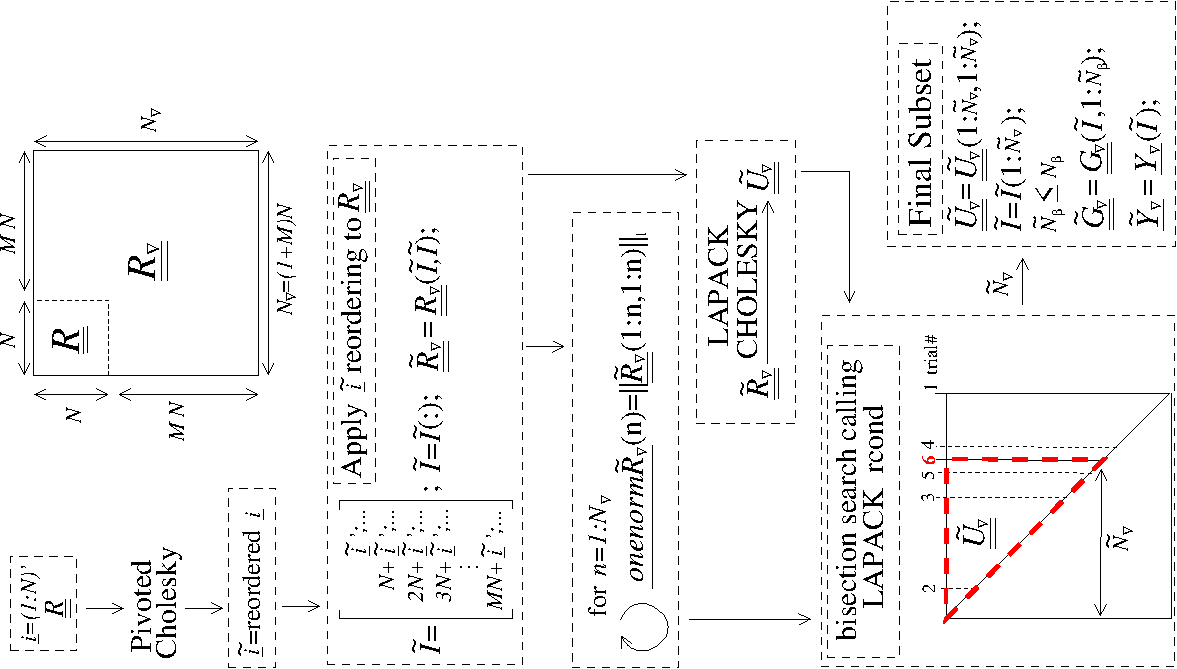
\includegraphics[width=6.9truein,angle=-90]{images/PivotCholSelectEqnAlgorithm.pdf}}
\caption{A diagram with pseudo code for the pivoted Cholesky algorithm used to select the subset of equations to retain when $\underline{\underline{R_{\nabla}}}$ is ill-conditioned. Although it is part of the algorithm, the equilibration of $\underline{\underline{R_{\nabla}}}$ is not shown in this figure.  The pseudo code uses MATLAB notation.}
\label{fig:SubsetSelectAlgorithm}
\end{figure}

To address computational efficiency and robustness, Dakota's pivoted
Cholesky approach for GEK was modified to: 
\begin{itemize}
\item Equilibrate $\underline{\underline{R_{\nabla}}}$ to improve 
      the accuracy of the Cholesky factorization; this is beneficial
      because $\underline{\underline{R_{\nabla}}}$ can be poorly 
      scaled. Theorem 4.1 of 
      van der Sluis \cite{Van69} states that if
      $\underline{\underline{a}}$ is a real, symmetric, positive 
      definite $n$ by $n$ matrix and the diagonal matrix 
      $\underline{\underline{\alpha}}$ contains the square roots of the 
      diagonals of $\underline{\underline{a}}$, then the equilibration
      \begin{displaymath}
        \underline{\underline{\breve{a}}}=\underline{\underline{\alpha}}^{-1}\underline{\underline{a}}\ \underline{\underline{\alpha}}^{-1},
      \end{displaymath}
      minimizes the 2-norm condition number of 
      $\underline{\underline{\breve{a}}}$ (with respect to solving linear 
      systems) over all such symmetric scalings, to within a factor of $n$.
      The equilibrated matrix $\underline{\underline{\breve{a}}}$ will 
      have all ones on the diagonal.
\item Perform pivoted Cholesky on $\underline{\underline{R}}$,
      instead of $\underline{\underline{R_{\nabla}}}$, to rank points 
      according to how much new information they contain.  This 
      ranking was reflected by the ordering of points in 
      $\underline{\underline{\tilde{R}}}$.
\item Apply the ordering of points in $\underline{\underline{\tilde{R}}}$
      to whole points in $\underline{\underline{R_{\nabla}}}$ to produce
      $\underline{\underline{\tilde{R}_{\nabla}}}$.  Here a whole point
      means the function value at a point immediately followed by the 
      derivatives at the same point.
\item Perform a LAPACK non-pivoted Cholesky on the equilibrated   
      $\underline{\underline{\tilde{R}_{\nabla}}}$ and drop equations off 
      the end until it satisfies the constraint on rcond.  LAPACK's rcond 
      estimate requires the 1-norm of the original (reordered) matrix as 
      input so the 1-norms for all possible sizes of 
      $\underline{\underline{\tilde{R}_{\nabla}}}$ are precomputed (using 
      a rank one update approach) and stored prior to the Cholesky 
      factorization.  A bisection search is used to efficiently determine 
      the number of equations that need to be retained/discarded. This
      requires ${\rm ceil}\left(\log2\left(N_{\nabla}\right)\right)$ or
      fewer evaluations of rcond.  These rcond calls are all based off the same
      Cholesky factorization of $\underline{\underline{\tilde{R}_{\nabla}}}$
      but use different numbers of rows/columns, $\tilde{N}_{\nabla}$.
\end{itemize}
This algorithm is visually depicted in Figure 
\ref{fig:SubsetSelectAlgorithm}.  Because inverting/factorizing a matrix 
with $n$ rows and columns requires $\mathcal{O}\left(n^3\right)$ flops, 
the cost to perform pivoted Cholesky on $\underline{\underline{R}}$ will be 
much less than, i.e. $\mathcal{O}\left((1+M)^{-3}\right)$, that of 
$\underline{\underline{R_{\nabla}}}$ when the number of dimensions $M$ 
is large.  It will also likely be negligible compared to the cost of
performing LAPACK's non-pivoted Cholesky on 
$\underline{\underline{\tilde{R}_{\nabla}}}$.

\section{Polynomial Models}\label{sec:poly_surr}

A preliminary discussion of the surrogate polynomial models available in
Dakota is presented in the Surrogate Models Chapter of the User's 
Manual~\cite{UsersMan}, with select details reproduced here. For ease of 
notation, the discussion in this section assumes that the model returns a 
single response $\hat{f}$ and that the design parameters $x$ have dimension $n$. 

For each point $x$, a linear polynomial model is approximated by
\begin{equation}
\hat{f}(x) \approx c_0 + \sum_{i = 1}^{n} c_i x_i,
\end{equation}
a quadratic polynomial model is 
\begin{equation}
\hat{f}(x) \approx c_0 + \sum_{i = 1}^{n} c_i x_i + \sum_{i = 1}^{n} 
\sum_{j \geq i}^{n} c_{ij} x_i x_j,
\end{equation}
and a cubic polynomial model is
\begin{equation}
\hat{f}(x) \approx c_0 + \sum_{i = 1}^{n} c_i x_i + \sum_{i = 1}^{n} 
\sum_{j \geq i}^{n} c_{ij} x_i x_j + \sum_{i = 1}^{n} \sum_{j \geq i}^{n}
\sum_{k \geq j}^{n} c_{ijk} x_i x_j x_k.
\end{equation}
In these equations, $c_0$, $c_i$, $c_{ij}$, and $c_{ijk}$ are the polynomial
coefficients that are determined during the approximation of the surrogate. 
Furthermore, each point $x$ corresponds to a vector $v_x$ with entries given 
by the terms $1$, $x_i$, $x_i x_j$, and $x_i x_j x_k$. The length $n_c$ of 
this vector corresponds to the number of coefficients present in the polynomial 
expression. For the linear, quadratic, and cubic polynomials, respectively,
\begin{eqnarray}
n_{c} 	&=& n+1, \\
n_{c} 	&=& \frac{(n+1)(n+2)}{2}, \\
n_{c}	&=& \frac{n^3 + 6n^2 + 11n + 6}{6}.
\end{eqnarray} 

Let the matrix $X$ be such that each row corresponds to the vector of a
training point. Thus, given $m$ training points, $X \in \mathbb{R}^{m \times
n_c}$. Approximating the polynomial model then amounts to approximating the
solution to
\begin{equation}
Xb = Y,
\end{equation} 
where $b$ is the vector of the polynomial coefficients described above, and $Y$
contains the true responses $y(x)$. Details regarding the solution or
approximate solution of this equation can be found in most mathematical texts
and are not discussed here. For any of the training points, the estimated
variance is given by
\begin{equation}
\sigma^{2}\left(\hat{f}(x)\right) = MSE\left(v_x^{T} (X^{T} X)^{-1} v_x\right),
\end{equation} 
where $MSE$ is the mean-squared error of the approximation over all of the
training points. For any new design parameter, the prediction variance is
given by 
\begin{equation}\label{eq:poly_var}
\sigma^{2}\left(\hat{f}(x_{new})\right) = MSE\left(1 + v_{x_{new}}^{T} 
(X^{T} X)^{-1} v_{x_{new}} \right).
\end{equation}
Additional discussion and detail can be found in~\cite{Net85}.



